%This is the fourth chapter of the dissertation

%The following command starts your chapter. If you want different titles used in your ToC and at the top of the page throughout the chapter, you can specify those values here. Since Columbia doesn't want extra information in the headers and footers, the "Top of Page Title" value won't actually appear.

\pagestyle{cu}
\graphicspath{{./Chapter4/Figures/}}
\chapter[Purity and the Electron Lifetime][Purity and the Electron Lifetime]{Purity and the Electron Lifetime}
\label{chap:purification}

In a noble element dark matter detection experiment the purity of the target mass is an essential consideration and must be measured
continuously.  To date the concentration of electronegative impurities has always been measured in these experiments, but no reliable
model has existed to explain and predict its behavior.

In this chapter I discuss the necessity of extremely pure xenon (\secref{}), explain the original model fit to XENON1T data
(\secref{}), and examine how abrupt changes in detector conditions alter the contamination (\secref{}).



\section{Importance and Procedure for Purifying Xenon}
\secref{sec:importance_procedure}
Purity usually refers to two distinct but correlated values, though the degree of the correlation can depend on the
experiment.  The first is radioactive elements of other noble elements that cannot be completely removed during distillation.  For xenon
our primary challenges are \ce{^{85}Kr} (\secref{subsubsec:backgrounds_electronic_krypton}) and \ce{^{222}Rn}
(\secref{subsubsec:backgrounds_electronic_radon}) as they have low-energy decays that can contaminate our region of interest (while
\ce{^{220}Rn} also leads to a low-energy \betadecay its half-life is too short to penetrate our detector and thus can be ignored).

The second consideration with regards to detector purity is contamination of electronegative impurities such as \ce{O_2} or
\ce{N_2}.  These attach to drifting electrons, lowering or even eliminating the S2.  This can have the largest impact at low energies
since the number of \electron is much fewer.  To correct for the expected initial number of electrons we can use the electron lifetime
$\tau_{\mathrm{e^-}}$, though this must be monitored consistently if not perpetually.  Of course, if the entire cloud of electrons is
removed by these impurities we cannot apply a correction since we have no knowledge of where in the detector it occurred or the energy
deposition.

This chapter is focused on the latter of these two purities, though its examination necessitates consideration of the former as we will
see.



\section{Effects of Electronegative Impurities}
\label{sec:importance_procedure_effects}
Impurities mainly come from outgassing of detector materials and diffusion of elements in the air surrounding the detector through seals,
though for the latter this is primarily limited to noble gases such as \ce{^{222}Rn} (\textbf{check this}).  While many of these
contribute to our electronic recoil background (\secref{subsec:backgrounds_electronic}) they can also decrease the number of photons and
electrons measured.

\subsection{Photon Attenuation}
\label{subsec:importance_procedure_effects_photons}
Contaminants been shown to absorb Xe scintillation (178 nm with ${\sim} 14\ \mathrm{nm}$ spectral FWHM)
(\citeref{Watanabe1953a, Watanabe1953b}).  At concentrations of ppm or higher
the fraction of UV photons that reach the PMTs can be considerably decreased - especially for large detectors.  The intensity due to
photon attenuation is given by

\begin{equation}
I(x) = I_0 e^{-x / \lambda_{\mathrm{att}}}
\end{equation}

\noindent where $I_0$ is initial intensity, $x$ is distance, and $\lambda_{\mathrm{att}}$ is the attenuation length.  It can be written
as $1 / \lambda_{\mathrm{att}} = 1 / \lambda_{\mathrm{abs}} + 1 / \lambda_{\mathrm{scatt}}$ where $\lambda_{\mathrm{abs}}$ and
$\lambda_{\mathrm{scatt}}$ are the the absorption and scatterings lengths, respectively.  For entirely pure xenon
$\lambda_{\mathrm{abs}} \sim \infty$ (\citeref{Baldini2005} found $lambda_{\mathrm{abs}} > 100\ \mathrm{cm}$ at 90\% confidence
level).

The inclusion of impurities, however, can shorten the absorption
length.  \figref{fig:importance_procedure_effects_photons_absorption_coefficents} shows the absorption coefficients
($\lambda_{\mathrm{abs}}^{-1}$) for 1 ppm \htwoo and \otwo from $130 \mdash 200\ \mathrm{nm}$.  They overlap with shorter wavelengths
of the xenon spectrum (included for comparison), meaning measured VUV photons by PMTs will not be symmetric above 178 nm.  With a nearly
1-meter tall detector a 1 ppm concentration of \htwoo would have an effect at 184 nm.

\begin{figure}
\centering
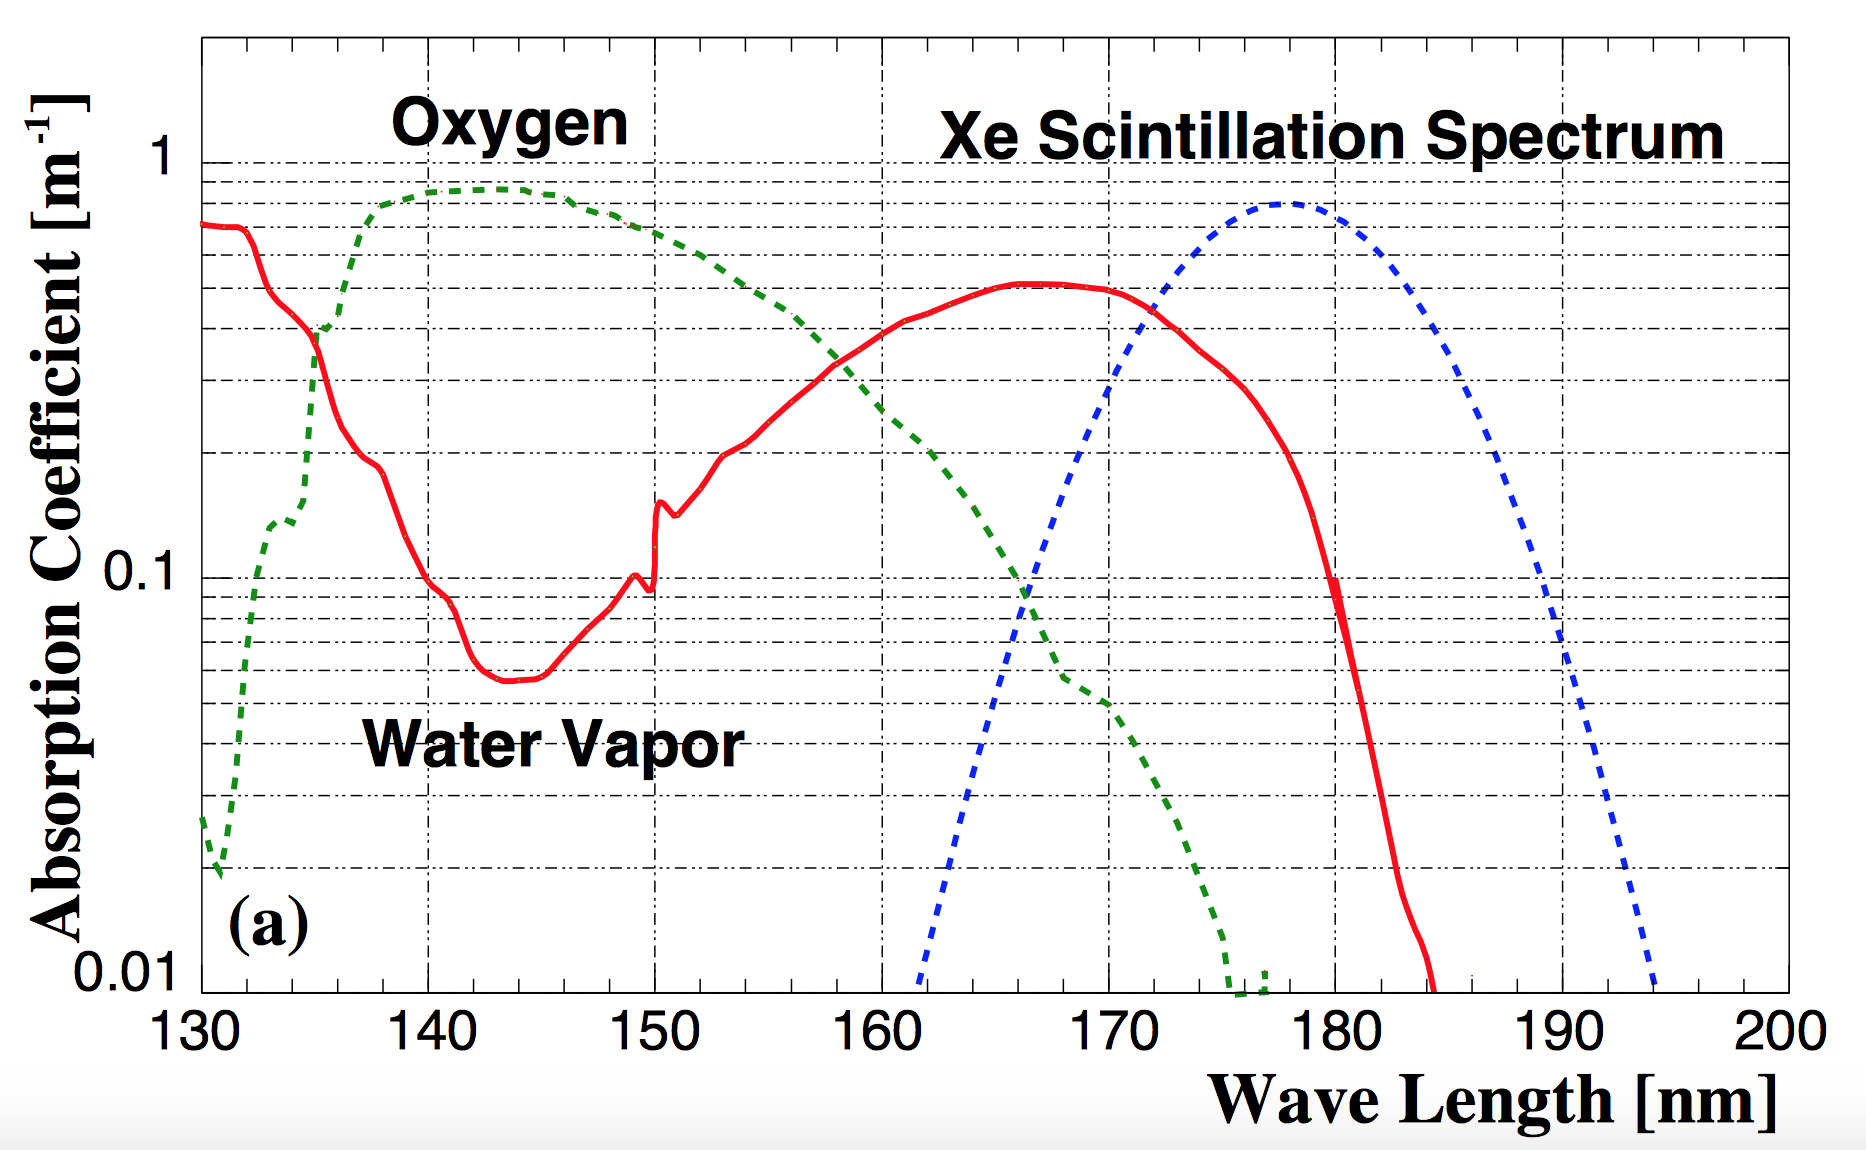
\includegraphics[width=0.8\textwidth]{AbsorptionSpectra}
\caption{Absorption coefficient for photons at 1 ppm \ce{H_2O} vapor (solid red) and \ce{O_2} (dashed green).  The Xe scintillation
spectrum is overlaid for comparison (dashed blue).  \ce{H_2O} impacts Xe scintillation considerably
more than \ce{O_2}.  Image credit: \citeref{Ozone2005}, \ce{H_2O} data from \citeref{Yoshino1996}.}
\label{fig:importance_procedure_effects_photons_absorption_coefficents}
\end{figure}

The relative intensities for different \ce{H_2O}/Xe and \ce{O_2}/Xe concentrations from $0 \mdash 60\ \mathrm{cm}$ are shown in
\figref{fig:importance_procedure_effects_photons_absorption_distance}.  We see that at the level of $\mathcal{O}(100)\ \mathrm{ppb}$ of
oxygen $I / I_0 > 0.8$ at 60 cm.  The effect of water is substantially worse with $I / I_0 < 0.3$, highlighting the necessity of
significant reduction in XENON1T.  Even with a LXe purity that is appreciably better than
\figref{fig:importance_procedure_effects_photons_absorption_distance} $\lambda_{\mathrm{att}} \sim \lambda_{\mathrm{abs}}$ since
the effects of scattering are subdominant with respect to absorption.

\begin{figure}
\centering
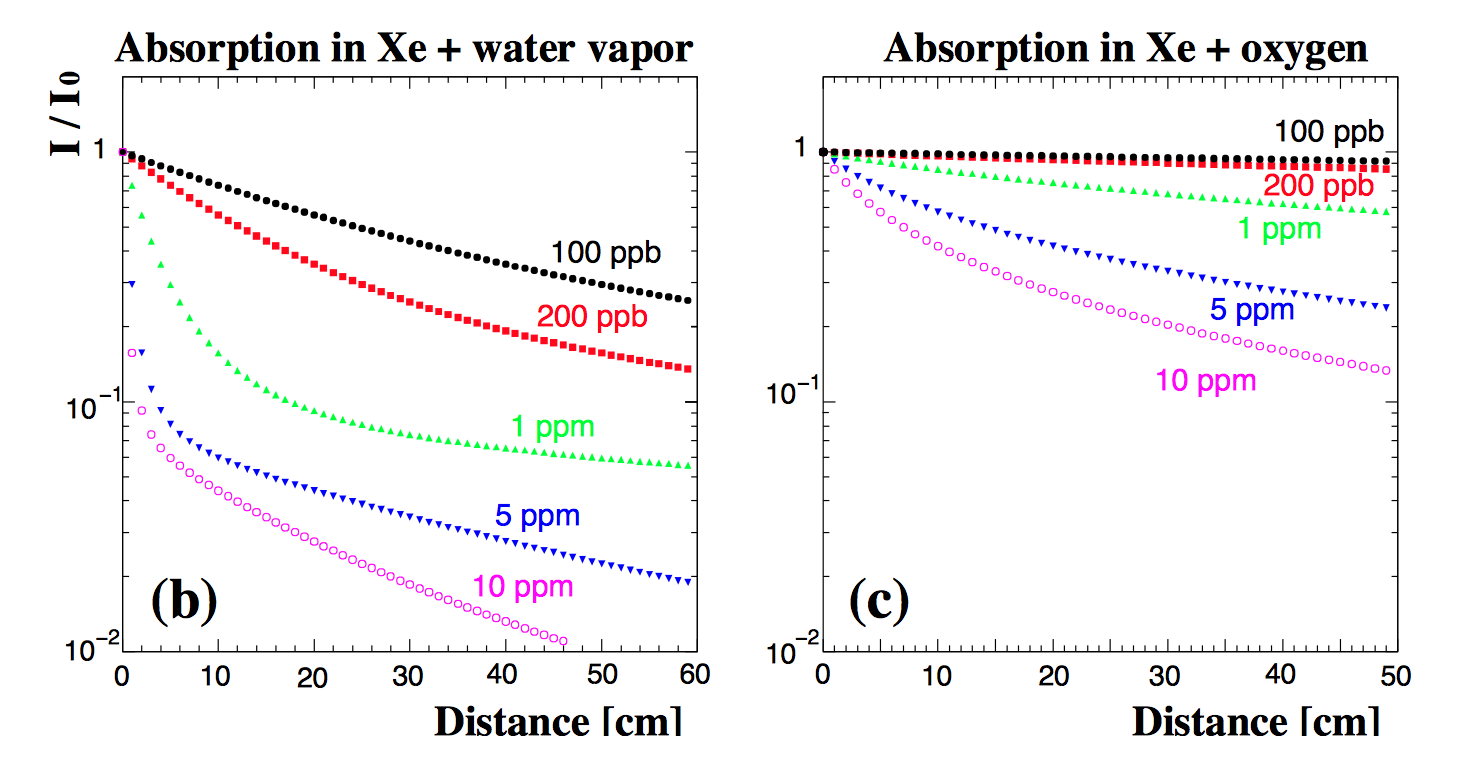
\includegraphics[width=\textwidth]{AbsorptionWithDistance}
\caption{Fraction of initial intensity of xenon scintillation with distance for various concentrations of \htwoo (left) and \otwo
(right).  Image credit: \citeref{Ozone2005}.}
\label{fig:importance_procedure_effects_photons_absorption_distance}
\end{figure}

Photon attenuation ultimately increases our energy threshold as we are less sensitive to lower energies as few photons are
measured.



\subsubsection{Charge Depletion}
\label{subsubsec:importance_procedure_effects_charge}
Electrons that do not recombine will drift antiparallel to $E_d$ in an electron cloud.  As the electron cloud drifts it diffuses both
longitudinally (in the direction of $E_{d}$) and transversely (perpendicular to $E_{d}$).  The
diffusion coefficients $D_{L}$ and $D_{T}$ are dependent on the electric field with $D_{T}/D_{L} \sim 10$.  The electron spread can
be written as $\sigma_{D_{T}} = \sqrt{D_{T} t_{d}}$ where $t_{d} = d/v_{d}$ is the drift time and $d$ is the drift distance.

The behavior of electrons can be classified according to their mobility in the limit of $E \rightarrow 0$, $\mu_0$.  When LXe is
polarized by electrons its high polarizability ($4.0 \times 10^{-24}\ \mathrm{cm^3}$, highest for noble gas) will both make it
attractive to \electron and interact with nearby Xe atoms through dipole-dipole interaction.  The equilibrium of these two effects
determines the potential energy of the ground state of electrons $V_0$, which is anti-correlated with $\mu_0$.  For LXe these have
been measured to be $V_0 = -0.61 \pm 0.05\ \mathrm{K}$ (\citeref{Tauchert1977}) and $\mu_0 = 2200 \pm 200\ \mathrm{cm^2\ V^{-1}\ s^{-1}}$
(\citeref{Yoshino1976}) at $165\ \mathrm{K}$ (in addition $\mu_0$ was found to be $1900$ and $2200\ \mathrm{cm^2\ V^{-1}\ s^{-1}}$
at $163\mathrm{K}$ by \citeref{Yoshino1976} and \citeref{Miller1968}, respectively).  The large electron mobilities indicate the
electrons are \textit{quasifree}, and have drift velocities that can exceed even those of GXe, as shown in
\figref{fig:importance_procedure_effects_charge_drift_velocity}.

\begin{figure}
\centering
\includegraphics[width=\textwidth]{drift_velocity_field}
\caption{Drift velocity (defined as $W$ here) dependence on reduced electric field $E/N$ where $N$ is the number of molecules per
volume.  Points are from experimental data (\citeref{Gushchin1982, Huang1978, Wagner1967, Pack1992}) and curves are from
calculations.  $1\ \mathrm{Td} = 10^-17\ \mathrm{V\ cm^2}$.  LXe has a higher drift velocity than GXe at
$E/N \lesssim 1\ \mathrm{Td}\ (1\ \mathrm{Td} = 10^{-17}\ \mathrm{V\ cm^2})$.  Image credit: \citeref{Atrazhev2005}.}
\label{fig:importance_procedure_effects_charge_drift_velocity}
\end{figure}

Ions exhibit significantly lower mobility than electrons.  It is parameterized as $\mu \approx \eta^{-\alpha}$ where $\eta$ is the
liquid viscosity and $\alpha = 1 \mdash 2$.  The diffusion coefficients can be calculated with the Nernst-Einstein equation

\begin{equation}
\frac{e D(E)}{\mu (E)} = \mathcal{F} <E>
\end{equation}

\noindent where $\mathcal{F} = 0.5 \mdash 1$ is depends on the electron distribution function (e.g. $\mathcal{F} = 2/3$ for a
Maxwellian distribution).

The mobilities for holes, \ce{TMSi^+}, \ce{O_2^-}, \ce{^{226}Th}, \ce{^{208}Tl}, and \ce{Xe_2^+} in in LXe are listed in
\tabref{tab:importance_procedure_effects_charge_mobilities}.  They are ${\sim} 10^6$ times smaller than the electron mobility.

\begin{table}
\centering
\begin{tabular}{cccccc}
Ion & T [K] & $\mu\ [10^{-4}\ \mathrm{cm^2\ V^{-1}\ s^{-1}}]$ & Ref. \\
\hline
holes & 161 & 35 & \citeref{Hilt1994b} \\
holes & 230 & 46 & \citeref{Hilt1994b} \\
\ce{TMSi^+} & 162 & 2 & \citeref{Hilt1994a} \\
\ce{TMSi^+} & 192 & 3 & \citeref{Hilt1994a} \\
\ce{O_2^-} & 162 & 6 & \citeref{Hilt1994a} \\
\ce{O_2^-} & 192 & 10 & \citeref{Hilt1994a} \\
\ce{^{226}Th^+} & 162 & 2.4 & \citeref{Wamba2005} \\
\ce{^{208}Tl^+} & 163 & 1.33 & \citeref{Walters2003} \\
\ce{Xe_2^+} & 184.2 & 2.85 & \citeref{Davis1962} \\
\ce{Xe_2^+} & 192.1 & 3.17 & \citeref{Davis1962} \\
\hline
\end{tabular}
\caption{Ion mobilities in LXe.  All ions listed are positive with the exception of \ce{O_2^-}.  Positive holes have mobilities that are
${\sim} 10$ greater than ions.  Summarized data is given in \citeref{Aprile2006a}.}
\label{tab:importance_procedure_effects_charge_mobilities}
\end{table}

Hole mobility can be described by the hopping model of charge carrier transport.  In this temperature-dependent model charge is
propagated through jumps between traps yielding

\begin{equation}
\mu = \frac{e b^2}{k_{\mathrm{B}} T} \omega
\label{eq:importance_procedure_effects_charge_mobility_simple}
\end{equation}

\noindent where $b$ is the average jump distance and $\omega$ is the jumping frequency, parameterized as

\begin{equation}
\omega = P \Big( \frac{\omega_0}{2 \pi} \Big) e^{-E_{\mathrm{a}} / k_{\mathrm{B}} T}
\end{equation}

\noindent where $\omega_0$ is the phonon frequency, $P(\omega_0 / 2 \pi)$ is the tunneling probability between adjacent holes with
activation energy $E_{\mathrm{a}}$.  \figref{importance_procedure_effects_charge_hole_mobility} shows hole mobility in
LXe.  The solid curve represents a model that parameterizes \eqref{eq:importance_procedure_effects_charge_mobility_simple} as

\begin{equation}
b^3(T) = \sqrt{2} M / \rho (T)
\end{equation}

\noindent where $M$ is the atomic mass of xenon and $\rho (T)$ is the temperature-dependent density (\citeref{Hilt1994b}).  It
additionally assumes the hole is self-trapped between two rare atoms in a potential well, forming a polaron.  It gives a hole mobility of

\begin{equation}
\mu (T) = \frac{e b^2 (T)}{k_{\mathrm{B}}} \frac{2 \pi}{h} \sqrt{\frac{\pi}{4 E_a k_{\mathrm{B}} T}} J_0^2
e^{-2 \alpha b(T)} e^{-E_a / k_{\mathrm{B}} T}
\label{eq:importance_procedure_effects_charge_mobility_polaron}
\end{equation}

\noindent where $h$ is Planck's constant and and $J(T) = J_0 e^{-\alpha b(t)}$ is the transfer integral.

\begin{figure}
\centering
\includegraphics[width=0.8\textwidth]{hole_mobility}
\caption{Fig. 3.15 in Aprile book.  Temperature-dependent drift mobility for holes in LXe.  Data is shown as empty triangles.  A fit
using \eqref{eq:importance_procedure_effects_charge_mobility_polaron} is shown as the solid line.  Image credit: \citeref{Aprile2006a}
(redrawn from \citeref{Hilt1994b}.)}
\label{fig:importance_procedure_effects_charge_hole_mobility}
\end{figure}

As the cloud drifts electronegative impurities can bond to \electron and prevent them from reaching the liquid-gas interface, thereby
decreasing proportional scintillation

\begin{equation}
e^{-} + S \rightarrow S^{-}
\label{eq:impurity_attach}
\end{equation}

\noindent where $S$ refers to the impurity (e.g. $e^- + \mathrm{O_2} \rightarrow \mathrm{O_2^-}$).

\begin{enumerate}
\item Radiative attachment is given by
\begin{equation}
e^- + XY \rightarrow XY^- + h \nu
\end{equation}

\noindent where $XY$ is some atom or molecule.

\item Dissociative electron attachment (DEA) is when a low-energy electron bonds to a molecule causing it to fracture.  The process
is given by

\begin{equation}
\begin{aligned}
e^- + XY \rightarrow XY^* + e^- \rightarrow X^+ + Y^- + e^- \\
e^- + XY \rightarrow XY^- \rightarrow X + Y^-
\end{aligned}
\end{equation}

\noindent where molecule $XY$ is separated into components $X$ and $Y$.  \ce{O_2} has 5.116 eV dissociation energy and \ce{O^-} has
electron affinity of 1.461 eV.

\item Three-body attachment proceeds via the two-stage Bloch-Bradbury reaction (\citeref{Bloch1935, Herzenberg1969})

\begin{equation}
e^- + XY \leftrightarrow (XY^-)* \\
(XY^-)^* + Z \rightarrow XY^- + Z
\end{equation}

\noindent where $Z$ is an atom or molecule from the majority gas population.  It carries out the bonding energy between the
\electron and electronegative $XY$.  Oxygen was studied (\citeref{Aleksandrov1993, Aleksandrov1981, Aleksandrov2009}).
\end{enumerate}



\section{Electron Lifetimes}
\label{sec:electron_lifetimes}
Nearly any mono-energetic radioactive decay can be used to measure the electron lifetime.  For XENON1T electron lifetimes were calculated
using the elements listed in \tabref{tab:electron_lifetimes_isotopes}.  An additional method of minimizing the \stwob band width using the
\ce{^{212}Pb} electronic recoil band to address an emerging discrepancy between
$\mathrm{^{83m}Kr}$ and \alphadecays (\secref{subsec:electron_lifetimes_rn222_vs_kr83m}) was tried but had too large of an uncertainty
to render itself valuable.

Following an \ambe or neutron generator calibration $\mathrm{^{129}Xe}$ and $\mathrm{^{131}Xe}$ will be in excited nuclear states
(\secref{subsubsec:electron_lifetimes_measurement_gammas}).  Their
$\gamma$-emissions and uniform distribution in the TPC make them excellent candidates to measure the electron lifetime for electronic
recoils.  Unfortunately their half-lifes of 8.88 and 11.93 d, respectively, eliminate any statistically significant results after more
than a few weeks.

\begin{table}
\centering
\begin{tabular}{rccrcc}
\hline
\hline
Isotope & Decay & Energy & $t_{1/2}$ & Section & Notes \\
\hline
$\mathrm{^{83m}Kr}$ & $\beta^-$ & $32.2\ \mathrm{keV}$ & 1.83 h & \secref{subsubsec:electron_lifetimes_measurement_kr} & Calibration \\
$\mathrm{^{129m}Xe}$ & $\gamma$ & $236.2\ \mathrm{keV}$ & 8.88 d & \secref{subsubsec:electron_lifetimes_measurement_gammas} & Background following NG cal. \\
$\mathrm{^{131m}Xe}$ & $\gamma$ & $163.9\ \mathrm{keV}$ & 11.93 d & \secref{subsubsec: electron_lifetimes_measurement_gammas} & Background following NG cal. \\
\ce{^{212}Bi} & $\alpha$ & $6.207\ \mathrm{MeV}$ & 60.55 m & \secref{subsubsec:electron_lifetimes_measurement_alphas} & \ce{^{220}Rn} calibration \\
\ce{^{218}Po} & $\alpha$ & $6.115\ \mathrm{MeV}$ & 3.10 m & \secref{subsubsec:electron_lifetimes_measurement_alphas} & Background (\ce{^{222}Rn} daughter) \\
\ce{^{222}Rn} & $\alpha$ & $5.590\ \mathrm{MeV}$ & 3.82 d & \secref{subsubsec:electron_lifetimes_measurement_alphas} & Background \\
\hline
\hline
\end{tabular}
\caption{Isotopes used for electron lifetime analysis.  Background \ce{^{222}Rn} and \ce{^{218}Po} \alphadecays allowed continual
monitoring of but had relatively low statistics.  $\mathrm{^{83m}Kr}$ and \ce{^{212}Bi} had high statistics but were only available during
calibrations.  Excited nuclear states $\mathrm{^{131m}Xe}$ and $\mathrm{^{129m}Xe}$ were present in background after nuclear recoil
calibrations but their half-lifes decreased viability after several weeks.}
\label{tab:electron_lifetimes_isotopes}
\end{table}



\subsection{Measuring the Electron Lifetime}
\label{subsec:electron_lifetimes_measurement}
The electron lifetimes over the XENON1T lifetime is shown in \figref{fig:electron_lifetimes_evolution_no_model}.  Initially lifetimes were
measured by selecting single-scatter data.



\subsubsection{S2/S1}
\label{subsubsec:electron_lifetimes_measurement_ss}
In the period immediately following XENON1T becoming operational the electron lifetime was ${\sim} 0$ since purification began at roughly
the same time.  The first in-situ calibration would not be performed until almost three months later and using any mono-energetic
background decays (which had not yet been investigated) would have given too few events in the top of the detector to be reliable.

Without being able to isolate any mono-energetic events S2 alone would be unable to establish the electron lifetime.  However,
S2/S1 - while not truly energy-independent - was enough so to give a reasonable estimate.  It was too early to have official cuts but
the ones used were sufficient and based on a history of knowledge of TPC detectors.

S1 (S2) single scatter cuts required that the second largest S1 (S2) be $< 0.2$ that of the first.  The purpose of these cuts was to
prevent S1-S2 mismatching: the S1 cut would
remove the possibility that we do not observe the S2 of a scatter deep in the TPC, while the S2 eliminated ambiguity in matching a single
S1 with two potential S2s.

To reject noise at least three PMTs must observe the S1.  This is the same cut that was used in the dark matter analysis.  Finally, the
fraction of light seen on the top PMT array must fall between $0.2 \mdash 0.6$ for S1s and $0.5 \mdash 0.9$ for S2s.

On a few occasions a \ce{^{137}Cs} was placed outside the detector.  While the LXe self-shielding limited the fraction of radiation that
made it inside the TPC enough events were present to get a dependable value.  This method was used until early August 2016.



\subsubsection{$\alpha$-Decays}
\label{subsubsec:electron_lifetimes_measurement_alphas}
The high energy and substantial stopping power (\figref{fig:mass_stopping_power}) of $\alpha$ interactions creates significant
recombination, in turn creating an S1 that makes them easily distinguishable from electronic and nuclear
interactions.  Because they are so recognizable and do not scatter many of the cuts developed for the science run analysis are not
necessary (many are in addition not reliable since they were developed using low-energy electronic recoils).  There are just a small
number of cuts that are used.

Events must have $r_{\mathrm{rec}} < 36.94\ \mathrm{cm}$.  This is in part for consistency with the First Results FV
(\citeref{Aprile2017f}).  But we can also expect inhomogeneity in the electric field to be greatest near the top, bottom, and sides of the
TPC as seen in \figref{fig:xenon1t_tpc_efield}.  Changes in the field would produce different light and charge yields
(\secref{subsec:det_char_ly_cy}), so the number $\gamma$s and escaped \electron would vary according to position.  Because $\alpha$
LY and QY have little dependence on field this effect is likely to be small or negligible.  However, a more alarming effect is impurity
attachment rate dependence on field, discussed in \secref{subsec:electron_lifetime_model_field}.  Finally, the radial cut removes any
chance of \alphadecays near the wall that would lose drifting \electron to the PTFE.

The fraction of light seen by the top PMTs from electroluminescence is tightly constrained due to the extraction occurring above the
liquid and over the roughly the same distance.  The percentage of events that fail this cut is small but it is important to remove any
``fake'' or gas-events (a cut on the S1 fraction seen by the top PMTs will also distinguish GXe events).

In addition data acquisition quality cuts are used in data selection.  The first is the high energy veto, which is triggered by a very
large S2.  The second is produced by one or more digitizers nearly filling its memory buffer, and is called a busy veto.  The third is
a busy type check, which removes events that have a busy signal anywhere in the waveform.  The final is an end of run check, which
disqualifies the last 21 per run (each run is 1 hour).  Details on each are given in \secref{subsec:xenon1t_daq}.

\figref{fig:electron_lifetimes_measurement_alphas_s1} shows S1 dependence on drift time for \alphadecays of \ce{^{222}Rn}
(${\sim} num\ \mathrm{PE}$) and \ce{^{218}Po} (${\sim} num\ \mathrm{PE}$) after these cuts.  The large
S1s from events deep in the detector can saturate PMTs in the bottom array, which lead to under-corrected cS1s as seen in the left
panel.  To correct for this the data are split into slices in $z$ and fit in cS1 with gaussians.  Fits in the region
$\lesssim z \lesssim$ where saturation is not present are interpolated to build a cS1 distribution, which is extrapolated across the
entire length of
the TPC.  Differences in fit parameters are used to relocate events deeper in the detector into the proper cS1 band.  The newly corrected
cS1 distribution is shown in the right panel of \figref{fig:electron_lifetimes_measurement_alphas_s1}.

\begin{figure}
\centering
\includegraphics[width=\textwidth]{s1_alpha}
\caption{cS1 (left) and $\alpha$-corrected cS1 (right) distributions with $z$.  The color and color boxes highlight \ce{^{222}Rn} and
\ce{^{218}Po} events, respectively.  In the left panel we can see severe distortion near the bottom of the detector.  Once corrected for
the effect is much less significant.}
\label{fig:electron_lifetimes_measurement_alphas_s1}
\end{figure}

Even with the $\alpha$-corrected cS1s we can still see there is saturation near the very bottom of the TPC.  The saturation is so great
here that events from \ce{^{222}Rn} and \ce{^{218}Po} cannot be distinguished from one another.  This is generally not a problem since it
is outside our fiducial volume.  There is also some distortion at $z \gtrsim$ from events
near the LXe surface, whose light is tightly concentrated in the top PMT array.

The selected \ce{^{222}Rn} and \ce{^{218}Pb} events are indicated by color and color boxes, respectively.  Events with $< z < $ and
$< \mathrm{cS1} < $ (\ce{^{222}Rn}) and $< \mathrm{cS1} <$ (\ce{^{218}Po}) are selected.  The electron lifetime is calculated for each
independent of the other, which provides a nice cross-check.  Because \ce{^{218}Po} has a half-life of just 3.1 m the number of events
should be roughly the same.  Each electron lifetime is calculated from 48 hours of data to get sufficient statistics.

The data is binned in $\delta t_d$ and an initial fit is performed on the 50th percentiles of the \stwob distributions from each
slice.  This preliminary electron lifetime $\tau_e^{(\mathrm{p})}$ is used to remove events that are far from the distribution.  The data
is then additionally binned in cS1 and fit with a gaussian in each $\delta t_d$ slice.  The means and standard deviations are then fit
with an exponential, yielding the final electron lifetime $tau_e$.  An example can be seen in
\figref{fig:electron_lifetimes_measurement_alphas_elifetime}.  The color (color) dashed lines define the boundaries above (below) which
events were cut with the preliminary fit.  Both fits are plotted in each panel for comparison.  We can see \ce{^{222}Rn} (left) and
\ce{^{218}Po} (right) give good agreement.

\begin{figure}
\centering
\includegraphics[width=\textwidth]{}
\caption{}
\label{fig:electron_lifetimes_measurement_alphas_elifetime}
\end{figure}

The overlap in \stwob highlights the necessity of using cS1 as a selection criterion.  Originally a cS1 $\alpha$-correction map did not
exist so \ce{^{222}Rn} and \ce{^{218}Po} were fit together.  This turned out to yield slightly lower $\tau_e$ than separate fits.  Once
the $\alpha$-correction was lifetimes was re-computed; however, this was not possible for some of the earlier data that had been
deleted.

This method can in principle be achieved for any $\alpha$-emitting element distributed throughout the FV of the detector and is done so
for \ce{^{212}Bi} during \ce{^{220}Rn} calibrations.


\subsubsection{$\mathbf{^{83m}Kr}$}
\label{subsubsec:electron_lifetimes_measurement_kr}
The delayed coincidence between the 32.2 and 9.4 keV decays help differentiate $\mathrm{^{83m}Kr}$ events from background.  With
$t_{1/2} = 154\ \mathrm{ns}$ for the 9.4 keV a large fraction of the S1s will overlap so a cut
$600 < \delta t_{\mathrm{S1}} < 2000\ \mathrm{ns}$
where $\delta t_{\mathrm{S1}}$ is the time between S1s is applied.  In addition we require the number of PMTs that see the 9.4 keV peak
to be $> 3$ to avoid coincident PMT noise and $< 30$ since it is low-energy.

The procedure to calculate the electron lifetime is similar to that described in
\secref{subsubsec:electron_lifetimes_measurement_alphas}.  An preliminary fit is performed using the median \stwob in each drift time
slice.  However, the high statistics and near-total background removal by the $\delta t_{\mathrm{S1}}$ cut
removes the need to exclude events far from the true \metakr.  Next each $\delta t_d$ slice is fit with a gaussian and an exponential
is then fit to the the results.



\subsubsection{$\mathbf{\gamma}$-rays}
\label{subsec:electron_lifetimes_measurement_gammas}
The full absorption peak of \gammarays make them great candidates for electron lifetime measurements.  Unfortunately nearly all
\gammarays in the TPC come from elements in detector materials or external sources placed inside the water tank
(e.g. \ce{^{137}Cs}).  However, nuclear recoils can excite \ce{^{129}Xe} and \ce{^{131}Xe} nuclei with half-lifes
of 8.88 and 11.93 days, respectively.  These metastable states serve as an in-situ calibration that can be used to measure a number of
detector parameters including light and charge yield (\secref{subsec:det_char_ly_cy}), $g_1/g_{2\mathrm{b}}$
(\secref{subsec:det_char_photon_charge_efficiencies}), and electron lifetime.  While these evaluations can validate fellow
electronic recoil measurements from \meta{83m}{Kr}, the short $t_{1/2}$ limit these to the few weeks following an \ambe or NG
calibration due.

Selecting \meta{129}{Xe} and \meta{131}{Xe} events is trickier than $\alpha$ or \meta{83}{Kr}.  This is in part because they sit
on top of an ER background (see \figref{fig:calibrations_photon_charge_efficiences_ces_resolution} for background energy spectrum), have a
relatively low event rate, and do not have properties that allow a high-percentage cut
efficiency (e.g. \meta{83}{Kr} delayed coincidence).  Instead a number of cuts need to be applied to remove unwanted data before a fit
can be done.

To select the 163.9 and 236.2 keV peaks an S2 single scatter cut is used to remove the underlying background.  Additional data quality
cuts include ensuring the fraction of the S2 seen by the top PMTs and the width of the S2 fall within known distributions.  For the FV
we apply the usual $r_{\mathrm{rec}} < 36.94\ \mathrm{cm}$ but require $-85 < z < -10\ \mathrm{cm}$ to remove \gammarays on the same
energy scale from surrounding materials that can penetrate deeper into the detector.

Because cS1 is known fitting the $\gamma$ peaks is reasonably simple, especially if the electron lifetime can be roughly estimated.  In
\figref{fig:electron_lifetimes_measurement_gammas_s1_s2} they are shown surrounded by contours from two-dimension gaussian fits.  The
y-axis is labeled as \cstwob because for this data $tau_e$ is known within small uncertainty - however, generally speaking this is not
the case.  The final cut we use then is to remove data outside some $\sigma$.

\begin{figure}
%    \centering
    \begin{subfigure}[t]{0.4\textwidth}
%        \centering
        \includegraphics[height=4cm]{}
    \end{subfigure}%
    \begin{subfigure}[t]{0.65\textwidth}
%        \centering
        \includegraphics[height=4cm]{}
    \end{subfigure}
    \caption{}
	\label{fig:electron_lifetimes_measurement_gammas_s1_s2}
\end{figure}

To verify the data we've selected is primarily \meta{129}{Xe} and \meta{131}{Xe} the event rate can be fit as seen in
\figref{fig:electron_lifetimes_measurement_gammas_decay_rate} shows the number of decays in the two months following the
SR0 \ambe calibration.  The fits give half-lifes that agree with the true values.  A constant is included to account for underlying
background.

\begin{figure}
\centering
\includegraphics[width=\textwidth]{xe_meta_decay_rate}
\caption{$\mathrm{^{129m}Xe}$ and $\mathrm{^{131m}Xe}$ events following the SR0 \ambe calibration.  Data is omitted during \metakr
and \ce{^{220}Rn} calibrations.  Fits using $R(t) = R_0 \mathrm{exp}(-t/t_{1/2}) + C$ give half-lifes of $8.66 \pm 0.26$ and
$11.51 \pm 0.43$ days, respectively, which match the known rates of 8.88 and 11.93 days.}
\label{fig:electron_lifetimes_measurement_gammas_decay_rate}
\end{figure}

The procedure to calculate $\tau_e$ is the same as in \secref{subsubsec:electron_lifetimes_measurement_alphas}.  The result for the
$num$ days following the \ambe calibration in \figref{fig:electron_lifetimes_measurement_gammas_decay_rate} (dateone to datetwo)
is shown in \figref{fig:electron_lifetimes_measurement_gammas_elifetime}.

\begin{figure}
\centering
\includegraphics[width=\textwidth]{}
\caption{Electron lifetimes using \meta{129}{Xe} and \meta{131}{Xe} 236.2 and 163.9 keV $\gamma$-rays.}
\label{fig:electron_lifetimes_measurement_gammas_elifetime}
\end{figure}

\begin{figure}
\centering
\includegraphics[width=\textwidth]{electron_lifetime_evolution_no_model}
\caption{Electron lifetimes of \ce{^{222}Rn} (color), \ce{^{220}Rn} (color), \ce{^{218}Po} (color), and \metakr (green circles) over the
XENON1T experiment.  We can see the lifetimes computed from \alphadecays differ from those of \metakr.}
\label{fig:electron_lifetimes_evolution_no_model}
\end{figure}



\subsection{\ce{^{222}Rn} vs. $\mathbf{^{83m}Kr}$}
\label{subsec:electron_lifetimes_rn222_vs_kr83m}
\figref{fig:electron_lifetimes_evolution_no_model} shows clear disagreement of electron lifetimes between $\alpha$-emitters and \metakr
at $\tau_e \gtrsim 400\ \mathrm{\mu s}$.  This presents a challenge for correcting \stwob for signals in the TPC.

The discrepancy is the result of field non-uniformity in the TPC (\figref{fig:xenon1t_tpc_efield}).  Because the change in recombination
of \alphadecays differs from that of electronic recoils (\figref{fig:tpcs_signals_drift_field}) the ratio of the \electron yields vary
inhomogeneously across the detector.  Thus two issues are apparent.  The first is bias will be present between any two events of equal
energy and type that occur at different fields in the detector.  Therefore we expect \metakr, $\mathrm{^{129m}Xe}$, and
$\mathrm{^{131m}Xe}$ to not accurately report the xenon purity.  The second is two events whose \electron yield changes in electric field
$dE/de^-$ are dissimilar require independent lifetime corrections.

In \figref{fig:electron_lifetimes_rn222_vs_kr83m_field_tpc} the electron yields for $\mathrm{^{129m}Xe}$ and \ce{^{222}Rn}
are shown throughout the TPC according to NEST (\citeref{NEST2013}). (assuming azimuthal symmetry).  The yields are normalized to the
region [$-90 \leq z \leq -85\ \mathrm{cm}$,
$r < 36.94\ \mathrm{cm}$].  The 1-ton fiducial volume is marked by the black line.  Both have decreasing yields in the $-z$ direction,
with the deviation for \ce{^{222}Rn} being more than twice as large as $\mathrm{^{129m}Xe}$.  This means $\tau_e$ is biased towards
smaller values but the effect is more significant for \ce{^{222}Rn} and other $\alpha$-decays.

Alphas are more sensitive to field changes.

\begin{figure}
\centering
\includegraphics[width=\textwidth]{relative_electron_yield_field_tpc}
\caption{Relative \electron yield with respect to [$-90 \leq z \leq -85\ \mathrm{cm}$, $r \geq 36.94\ \mathrm{cm}$] for
$\mathrm{^{129m}Xe}$ (left) and \ce{^{222}Rn} (right) for ${\sim}120\ \mathrm{V\ cm^{-1}}$ inside the 1T FV (black line).  A decline in
yield is
observed moving in the $-z$ direction, which leads to a misleading observation that the electron lifetime is lower than its true
value.  The imbalance between the top
and bottom of the TPC is $\gtrsim 2\times$ larger for \ce{^{222}Rn}, causing it to appear lower than its $\gamma$ counterparts.}
\label{fig:electron_lifetimes_rn222_vs_kr83m_field_tpc}
\end{figure}

The $z$-dependence of \electron yields for $\mathrm{^{129m}Xe}$, $\mathrm{^{131m}Xe}$, \ce{^{60}Co}, \ce{^{208}Tl}, and \ce{^{222}Rn} is
plotted in \figref{fig:electron_lifetimes_rn222_vs_kr83m_field_z} (averaged over $r < 36.94\ \mathrm{cm}$).  The NEST results are
normalized to the same region as \figref{fig:electron_lifetimes_rn222_vs_kr83m_field_tpc}.  \ce{^{60}Co} and \ce{^{208}Tl} (1173.2 and
2614.5 keV, respectively) are shown for comparison with lower-energy metastable xenon.  The difference in relative yields is small but
may explain the minor inconsistencies at higher energies in \figref{fig:calibrations_photon_charge_efficiences_ces_resolution}.  The
effect of \ce{^{222}Rn} is more substantial and demonstrates that calculations of $\tau_e$ - which depend on slices in $z$ - suffer from
bias as a result of inhomogeneous recombination derivative dependence on field.  The higher sensitivity of \alphadecays explains
the lower lifetime measured, though a separate field-dependent effect also needs consideration and is discussed in
\secref{subsec:electron_lifetime_model_field}.

\begin{figure}
\centering
\includegraphics[width=\textwidth]{relative_electron_yield_field}
\caption{Relative electron yield dependence on $z$ with respect to the region $-90 \leq z \leq -85\ \mathrm{cm}$ and
$r \geq 36.94\ \mathrm{cm}$ using NEST (\citeref{NEST2013}).  Internal $\gamma$ sources $\mathrm{^{131m}Xe}$ (green) and
$\mathrm{^{129m}Xe}$
(red) are shown, with higher energies \ce{^{60}Co} (black) and \ce{^{208}Tl} (pink) plotted for comparison.  We can see their relative
light yield varies by ${\sim} 5\%$, with the higher-energy lines having only ${\sim} 1\%$ greater difference than $\mathrm{^{131m}Xe}$ and
$\mathrm{^{129m}Xe}$.  \ce{^{222}Rn} (blue) changes by $> 10\%$.  The disproportionate growth demonstrates that the ratio between
$\alpha$ and $\gamma$ electron yields is largest at the top of the detector, causing the fewer \electron from deep \alphadecays to
mimic a smaller $\tau_e$.  \metakr cannot be compared as the NEST version is only for high-energy.}
\label{fig:electron_lifetimes_rn222_vs_kr83m_field_z}
\end{figure}



\section{Electron Lifetime Model}
\label{sec:electron_lifetime_model}
To construct the electron lifetime model a number of factors were considered.  The model was fit to the \ce{^{222}Rn} $\alpha$-emissions
due to its constant presence in our background.  The best-fit trend was then scaled to match the $\mathrm{^{83m}Kr}$ data using a derived
``correction function'' to correct electronic recoil science data (\secref{subsec:electron_lifetimes_rn222_vs_kr83m}).



\subsection{Columbia Demonstrator}
\label{subsec:electron_lifetime_model_demonstrator}
To address new challenges in upgrading to a ton-scale detector a prototype was constructed at Columbia.  While much smaller in total
volume (${\sim}26\ \mathrm{kg}$ total, ${\sim}4\ \mathrm{kg}$ inside TPC) part of its goals were to assess the feasibility of 1-meter
drift lengths, which in turn required a significant improvement in xenon purification compared to the ${\sim}5\ \mathrm{slpm}$ of its
predecessor XENON100 (\citeref{Aprile2012a}).

\begin{figure}
\centering
\includegraphics[width=0.8\textwidth]{fig_1_Aprile2012b}
\caption{Schematic of the Columbia Demonstrator in its initial state.  The connection to bring GXe to the getter was not yet installed
at the time of publication (\secref{subsec:electron_lifetime_model_gxe}).  Image credit: \citeref{Aprile2012b}.}
\label{fig:electron_lifetime_model_demonstrator_schematic}
\end{figure}



\subsection{Impurity Removal}
\label{subsec:electron_lifetime_model_removal}
See if purification system diagram exists for after magnetic pump installed.

Impurities are removed in the purification system (\citeref{subsec:xenon1t_pur}) by two SAES PS4-MT50-R getters.  It operates between
$5 \mdash 100\ \mathrm{slpm}$ and uses heated zirconium ($400^{\circ}\mathrm{C}$ nominal operating temperature) to form irreversible
chemical bonds with \ce{O_2}, \ce{CO}, \ce{CO_2}, \ce{H_2O}, \ce{H_2}, \ce{N_2}, and \ce{CH_4}, achieving levels of
$< 1\ \mathrm{ppb}$.

\begin{figure}
\centering
\includegraphics[width=0.8\textwidth]{LT_cycle_all-eps-converted-to}
\caption{Electron lifetime dependence on flow rate through getter.  Measurements are done for 5 (pink circles), 20 (blue squares), 30
(blue
triangles), 41 (green triangles), 50 (red squares), and 80 (black circles) slpm.  With the exception of the 5 slpm, the lifetimes increase
at roughly the same rate ($\lesssim 7\ \mathrm{cycles}$).  From 0 to 50 slpm an increase in flow produces a higher ultimate electron
lifetime.  At 80 slpm the $\tau_e$ drops below 50 slpm.  An explanation may be that at high speeds impurities cannot be removed as
efficiently due to the short time spent in the getter.  Image credit: \citeref{Demonstrator2018}.}
\label{fig:electron_lifetime_model_removal_demonstrator_circ}
\end{figure}

An SAES PS4-MT50-R1 getter was installed in the Columbia Demonstrator for testing.



\subsection{Vaporization and Condensation}
\label{subsec:electron_lifetime_model_vap_and_cond}
Impurities will transfer between the gas and liquid xenon.



\subsection{GXe Purification}
\label{subsec:electron_lifetime_model_gxe}
Because only the electrons drifting in the LXe lead to an S2 purifying the GXe was historically not considered necessary.  However,
the relatively light mass of electronegative impurities with respect to xenon and higher temperatures that produce greater outgassing
suggest that many more may be present in the gas.  Because
impurities are exchanged between the liquid and gas (\secref{subsec:electron_lifetime_model_vap_and_cond}) the potential to compromise
the electron lifetime is significant.

As part of the work leading up to XENON1T the Columbia Demonstrator installed piping connecting the gaseous region of the TPC to the
purification system to investigate this effect.  \figref{fig:electron_lifetime_model_gxe_demonstrator} shows the electron lifetimes over
the course of the measurement using a \ce{^{137}Cs} 661.7 keV $\gamma$-ray.  Two periods with GXe and LXe circulation were observed and
are highlighted in blue.  Each shows an increase in
$\tau_e$, though the second was only for a few days.  The first measurement improves the lifetime from
${\sim} 200 \mathrm{\mu s}$ to ${\sim} 450 \mathrm{\mu s}$ and does not show signs of leveling off when the LXe-only circulation is
restored.  This confirmed the expectation that electronegative impurities in the GXe play an important role in limiting the electron
lifetime, and our dark matter search would benefit greatly from equipping XENON1T for GXe purification.

\begin{figure}
\centering
\includegraphics[width=\textwidth]{eLT_gas_rec}
\caption{Electron lifetime with (white) and without (blue) GXe circulation for the Demonstrator.  The electron lifetime more than doubles
in the first iteration over a roughly 10-day span.  A period follows with
only LXe purification, but is too short to observe much decrease.  Upon re-initiating GXe flow the lifetime drops a bit - possibly due to
trapped impurities in the GXe tubing - but then begins to climb again.  The final block reveals the electron lifetime does
decrease with LXe-only circulation.  Image credit: \citeref{Demonstrator2018}.}
\label{fig:electron_lifetime_model_gxe_demonstrator}
\end{figure}

Three lines were connected to the GXe region of the XENON1T - one at each cooling tower
(\figref{fig:xenon1t_cryogenics_schematic,fig:xenon1t_cryo_overview}) - to siphon gas to the purification system
(\secref{subsec:xenon1t_pur}).  As the highest and warmest regions in the detector the impurity concentrations were predicted to be
significant.  A fourth conduit is linked to the tube that carries the cables between the TPC and data acquisition, where contamination
is expected to be higher from outgassing as a result of the inability to apply the same cleaning standard as other detector materials
(\textbf{check this}).

During standard operations GXe is passed through the getters at ${\sim} 3.75\ \mathrm{slpm}$, or roughly $7 \mdash 8\%$ of the total
flow during SR0 and SR1.

From August 22 to September 2, 2016 LXe purification was halted.  The motivation was to study the effect that GXe purification has by
decoupling it from the liquid.  We found the electron lifetime decreased more rapidly than anticipated, indicating that while the
impurities in the GXe were influential, they were not to the extent predicted.  The GXe-only circulation provides unique insight into
the physics of impurity behavior in a TPC.  Correctly modeling this portion of the evolution constrains the outgassing, vaporization,
and condensation rates.



\subsection{Outgassing and Leaks}
\label{subsec:electron_lifetime_model_outgassing}



\subsection{Field Dependence}
\label{subsec:electron_lifetime_model_field}



\subsection{Detector Effects}
\label{subsec:electron_lifetime_model_detector_effects}



\subsubsection{Getter Defficiencies}
\label{subsubsec:electron_lifetime_model_detector_effects_getter}



\subsubsection{Impurity Spikes}
\label{subsubsec:electron_lifetime_model_detector_effects_spikes}



\subsection{Operations}
\label{subsec:electron_lifetime_model_ops}

\begin{figure}
\centering
\includegraphics[width=\textwidth]{pur_system_mag_pump_upgrade}
\caption{}
\label{fig:mag_pump}
\end{figure}

Electronegative impurities
in particular present a problem
since they attach to drifting $e^{-}$,
lowering the number that reach the liquid-gas interface and thus decreasing the secondary scintillation.  The attachment process
is \eqref{eq:impurity_attach}.

Discuss 100 SLPM plan and choking by pipes, why didn't reach it.  \ce{^{222}Rn} decrease with magnetic
pump.  Connect to Demonstrator - attempt to drift electrons 1 meter.  Make clear why it's so important.  Discuss how much lose in
sensitivity.  Tests to understand individual components.  Include flow model by Guillaume, what we hope to achieve using it.  Show
waveforms for same energy event - one at top and one at bottom of detector and how bottom is worse.  Discuss qualitatively electron
lifetime before discuss model.

\noindent where $S$ is the impurity.  The number of \electron captured is dependent drift time $t_{d}$ and the
attachment rate of
the impurities $k_{S}$, both of which depend on $E_{d}$.  Clearly then an advantage of larger
\efields is a larger
\vd (up to a point, see \figref{fig:drift_velocity}) and thus less time in the liquid.  Doping LXe with organic materials such as butane
can increase \vd at stronger
\efields but are not used in DM detectors due to difficulty in purifying (\citeref{Yoshino1976}).  The rate at which electrons are
absorbed by impurities is proportional to the number of electrons, impurities, and impurity attachment rate.  Assuming the the density
of impurities in the liquid and $E_{d}$ are uniform we find

In an electric field $E$ an \electron that is freed but does not recombine with its parent or other ionized atoms will move anti-parallel
to the field at drift velocity $v_{d}$.  At fields of $\lesssim 100\ \mathrm{V\ cm^{-1}}$ drift velocity is nearly proportional to
$E$ and is given by $v_{d} = \mu E$
where $\mu$ is the electron mobility.  For this energy region $\mu \sim 2200\ \mathrm{cm^{2}\ V^{-2}\ s^{-1}}$ (\citeref{Yoo2015}).  As
$E$ increases $v_{d} \propto E^{1/2}$ and ultimately flattens at $\sim 3\ \mathrm{mm\ \mu s}$.  \figref{fig:drift_velocity} shows \vd
as a function of $E$ and \tabref{tab:drift_velocity} gives the approximate relationship.

The strength of $E$ affects the number of electrons freed, as a larger field decreases
recombination electron-ion recombination.  In liquid noble gas detectors used for DM searches such a field can be used to drift the
\electron to the surface of the liquid, where they are extracted across a small region of gas.  Doing so will produce secondary
scintillation as the \electron will energize the atoms in the gas, freeing more \electron in turn.  Because the amount of scintillation
produced per electron is independent of the number of electrons extracted this is also known as proportional scintillation.  Thus, by
measuring this scintillation the number of \electron extracted can be determined.  Details of \electron drift and proportional
scintillation is found in \secref{subsec:tpcs_working_principle}.

For $E \lesssim 100\ \mathrm{V\ cm^{-1}}$ \vd$\propto E$, $100 \lesssim E \lesssim 10^{3 \ mdash 4}$
\vd$\propto E^{1/2}$, and $E \gtrsim 10^{4}$ \vd plateaus at $\sim 3\ \mathrm{mm\ \mu s^{-1}}$ (\citeref{Miller1968}).

\begin{table}
 \centering
 \begin{tabular}{cc}
 \hline
 $E$ [V cm$^{-1}$] & \vd [mm $\mu$s$^{-1}$] \\
 \hline
 $\lesssim 100$ & \vd$\propto E$ \\
 $\sim 100 \mdash 10^{3 \mdash 4}$ & \vd$\propto E^{1/2}$ \\
 $\gtrsim 10^{4}$ & \vd$\sim 3$ \\
 \hline
 \caption{Drift velocity \vd dependence on electric field for LXe.}
 \end{tabular}
 \label{tab:drift_velocity}
\end{table}

\begin{figure}
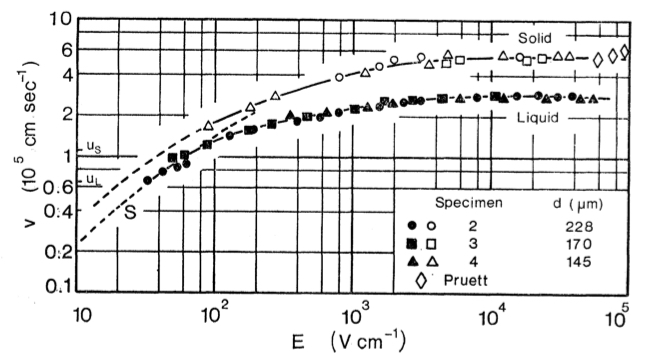
\includegraphics[angle=0.5, width=0.8\textwidth]{DriftVelocity}
\caption{Drift velocity for solid and liquid xenon}
\label{fig:drift_velocity}
\end{figure}
In addition to absorbing VUV photons impurities can attach to drifting electrons.






Page 257 in Aprile book